\chapter{Averaged equations and popualtion balance equations}
\label{chap:avg}

In this chapter we summarize the theoretical framework available to average two phases flows equations. 
In the first place we introduce the different parameters of the problem at hands and the governing equations. 
Then, we present averaging methods for a two-phase flow with no assumption \textit{ad-hoc}.  
Afterwards, we go into deeper details about the closures terms of these equations, and debrief on the usefulness of these terms into an Euler-Euler model. 
We investigate the different models available for specific cases (e.g. solid and spherical particles, non-spherical particles\ldots).
After noticing that there is a lake of models regarding deformable particles, we derive an averaged equation for the dispersed phase considering deformations of the particles and discuss its utility.
In a second part we make an overview of all the numerical studies investigating on the closures terms. 
We then conclude on the main results of those studies and deduce the remaining subjects to investigate. 

\section{Physical parameters and Governing equations for two phases flows}
In the core of the report all the physical parameters refer to the ones presented in this section.
As mentioned in \ref{chap:intro} we aim to model an emulsion, thus the theoretical problem is a two phase flow problem with a dispersed phase immersed in a continuous phase. 
On the \ref{fig:scheme} we can observe the scheme of the situation. 
We define the droplet viscosity with $\mu_d$ and density with $\rho_d$.
The size  of a droplet  $\alpha$ (which isn't necessarily the diameter) is noted by $L^\alpha$. 
The average representative length is the mean of the $L^\alpha$ noted $\bar{L}$. 
The continuous phase has a viscosity $\mu_f$ and density $\rho_f$.
The only external force that we will consider is the gravity $\bm{g}$. 
\begin{figure}
    \centering
    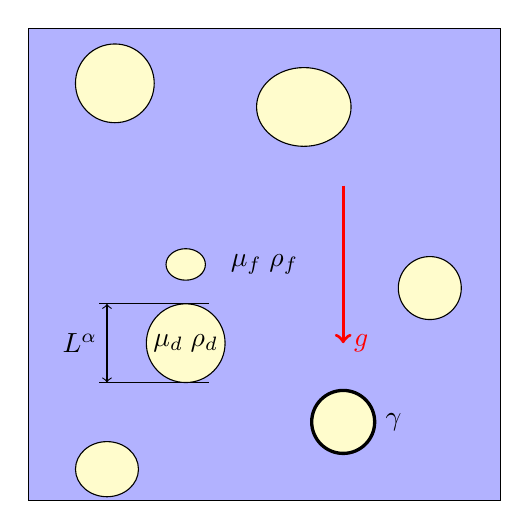
\begin{tikzpicture}
        \draw[fill=blue!30](0,0) rectangle(6,6);
        \draw[fill=yellow!20](3,3) node{$\mu_f\;\rho_f$};
        \foreach \x/\y/\ra/\r in {2/3/0.2/0.25,5.1/2.7/0.4/0.4,1/0.4/0.35/0.4,4/1/0.4/0.4,3.5/5/0.5/0.6,1.1/5.3/0.5/0.5}{
            \draw[fill=yellow!20](\x,\y) ellipse(\r cm and \ra cm);
        }
        \draw[fill=yellow!20](2,2) circle(0.5)node{$\mu_d\;\rho_d$};
        \draw[thin,-](0.9,2.5)--++(1.4,0);
        \draw[thin,-](0.9,1.5)--++(1.4,0);
        \draw[very thick,black!80!black](4,1) ellipse (0.4cm and 0.4cm);
        \draw[very thick,black!80!black](4,1)++(0.4,0)node[right]{$\gamma$};
        \draw[thin,<->](1,1.5)--++(0,1)node[midway,left]{$L^\alpha$};
        \draw[very thick,->,red](4,4)--++(0,-2)node[right]{$\bm{g}$};
    \end{tikzpicture}
    \caption{Scheme of droplets immersed into a fluid.}
    \label{fig:scheme}
\end{figure}
We now introduce the phase indicator function :
\begin{equation}
    \chi(\bm{x}) = \left\lbrace \begin{tabular}{c}
        $1 \;\text{if}\; \bm{x} \in V_d$\\
        $0 \;\text{if}\; \bm{x} \in V_f$\\
    \end{tabular}\right.,
\end{equation}
with $\bm{x}$ the position vector, $V_d$ the volume occupied by the dispersed phase and $V_f$ the one occupied by the continuous phase or fluid phase. 
At the interface of the droplets and fluid we can observe a superficial surface tension that we will refer to as $\gamma$.

There is a total of $7$ physical parameters to this problem, they are all constituted by 3 fundamental units, a length, a mass and a time.
Therefore,, according to Buckingham $\pi$ theorem we can define a minimum of $7-3 = 4$ dimensionless number to describe the physics. 
Several options are available, but we choose the following one: 
\begin{equation*}
    Ar = Ga^2 =\frac{\rho_f(\rho_f - \rho_d) g \bar{L}^3}{\mu^2_f},
\end{equation*}
\begin{equation*}
    Eo = Bo =\frac{(\rho_f - \rho_d) g \bar{L}^2}{\sigma},
\end{equation*}
\begin{equation*}
    \mu_r = \frac{\mu_d}{\mu_f}
\end{equation*}
\begin{equation*}
    \phi = \frac{V_d}{V_f}
\end{equation*}
The \textit{Galileo number} or \textit{Archimedes number}, is the ratio of the buoyancy forces over the viscosity forces.
Note that the \textit{Reynolds number}, $Re = \rho_f L U/\mu$, where $U$ is the characteristic velocity, is equivalent to the \textit{Galileo number} if we take the velocity scale $U = \sqrt{gL(\rho_f-\rho_d)/\rho_f}$.
$Bo$ is the \textit{Bond} or \textit{Eötvös number}, it is the ratio between the buoyancy forces and surface tension forces. 
$\mu_r$ is the ratio of viscosity and $\phi$ the Volume fraction of the dispersed phase.
Note that $We^2 = Bo/Ga^2$, with $We$ the \textit{Weber number} which compare the viscous forces with capillarity forces.
$We$ will somewhat describe the deformation of the drops. 
To give a brief idea about the values of those number in the real application let's take the example of an oli/water emulsion.
In the real processes the diameter of the droplets $L = [10 \mu m, 1 mm]$.
The density and viscosity of water are respectively $\rho_f = 1000 kg/m^3$ and $\mu_f = 10^{-3}$.
The density and viscosity of oil are $\rho_d = 900 kg/m^3$ and $\mu_d = 10^{-2}$.
We consider the gravity acceleration on earth, it is $g= 9.81 kg.m.s^{-2}$.
The surface tension of the system oil/water is $\sigma = 50 mJ/m^2$ \citep{de2015gouttes}. 
Then, we can observe the values of dimensional parameters \ref{tab:parameters}.
\begin{table}[h!]
    \centering
    \begin{tabular}{|c||c|c|c|c||||c|}
        \hline&$Ga$&$Bo$&$\phi$&$\mu_f/\mu_d$&$We=\sqrt{Bo}/Ga$\\ \hline
        \hline Oil/Water&$[0.03,30]$&$[10^{-6};10^{-2}]$&$\phi$&$0.1$&$ $\\ \hline
    \end{tabular}
    \caption{dimensionless parameters for a water/oil emulsion}
    \label{tab:parameters}
\end{table}


\subsection{Governing equations}
Now, let's introduce the mass and momentum balance for two fluid flows. 
There are two possible formulations to express the conservation principle in two phase flow \citep{tryggvason2011direct}, in the following a brief summary of the two methods.

\subparagraph*{Two-fluid formulation :} In this formulation we explicitly include equations to describe the stress jump and velocity continuity at the interfaces.
Therefore,, this model includes the equation of conservation of mass, it reads,
\begin{equation}
    \label{eq:Cmass}
    \bm{\nabla} \cdot \bm{u}= 0,
\end{equation}  
with $\bm{u}$ the velocity fields.
The conservation of momentum reads as,
\begin{equation}
    \label{eq:Cmomentum}
    \rho \frac{D \bm{u}}{Dt} = \bm{\nabla} \cdot \bm{\sigma} + \bm{b},
\end{equation}
with $\frac{D ()}{Dt}  =  \frac{\partial ()}{\partial t}  + \bm{u} \bm{\nabla} \cdot ()$, $\bm{\sigma}$ is the stress tensor and $\bm{b}$ the body forces including the gravity. 
The material property $\rho$ and $\mu$ takes the values of the present phase thus we drop the indices.  
Then, in order to well define the physics at the interface we need two additional equations. 
Namely, the velocity continuity at the interface,
\begin{equation*}
    \left[\bm{u}\right]_S = 0
\end{equation*}
where $[x]_S$ is the jump notation $ [x]_S = x_d-x_f$.
And the stress continuity equation,
\begin{equation*}
    \underbrace{-[\bm{\sigma}]_S}_{\text{Stress jump}} \cdot \bm{n} = \underbrace{\gamma \kappa \bm{n} +\nabla_S \gamma}_{\text{Surface force}},
\end{equation*}
where $\bm{n}$ is the outward normal at the interface, $\nabla_S$ the surface divergence operator and $\kappa$ is the curvature of the interface defined by $-\bm{\nabla}_S\cdot\bm{n}$. 
We can note that the surface force include a term as the divergence of $\gamma$, which is supposed to account for non-constant superficial surface tension.
However, We will neglect this term in what follow, thus we define the surface force as $\bm{f_\gamma} = \gamma \kappa \bm{n}$.
\subparagraph*{One-fluid formulation :} This formulation require no additional equations instead a body force is added to the momentum balance. 
Therefore,, in this model we consider only \ref{eq:Cmass} and the following equation,
\begin{equation}
    \label{CmomentumOnefluide}
    \rho \frac{D \bm{u}}{Dt} = \bm{\nabla} \cdot \bm{\sigma} + \bm{b} + \bm{f_\gamma} \delta_S ,
\end{equation}
where $\delta_S = \delta(\bm{x} - \bm{x}_S)$ with $\delta$ the Dirac delta function and $\bm{x}_S$ the positions of the interface.

In the two-fluid approach the surface tension is taken in account though the boundary condition. 
It is mostly used in theoretical developments, while averaging the equations for example.
While, in the letter it is included as a body forces term in the momentum conservation equation. 
This formulation allows a greater ease to implement multiphase flows into DNS code since there is no boundary condition at the interface.
More details on the numerical methods will be provided in the \ref{chap:DNS}. 

\subsection{Phenomenology of drops/bubbly flows.}
\textcolor{blue}{should i let this part or not ?}
\textbf{In this section depict all the physical aspect of a bubbly flow, here are some examples.}
Depending on the physical parameters the drops are more likely to arrange them self to line up horizontal "raft" or in column \citep{tryggvason2011direct}\citep{guazzelli2011}. 

\citet{morel2010comparison} The larger bubbles tend to go toward the axis while the smaller outward of the bubble columns.


\section{Averaged Navier-Stokes equations for dispersed two phase flows}

As stated in \ref{chap:intro} it is impossible to resolve \ref{eq:Cmass} and \ref{eq:Cmomentum} with DNS, at the industrial scale. 
Moreover, the microscale interactions is not relevant to optimize these processes, only the macroscopic quantities matters. 
Therefore,, we need laws that describe the macroscopic scale without solving the expensive two-fluid problems. 
This is the aspiration of averaging or Up-scaling technics.
Indeed, by averaging a given representative volume we can derive macro-scale equations of conservation for the mean quantities, such as the averaged velocity fields and averaged pressure fields. 
This way we do not have to solve the microscale.
Nevertheless, the macro-scale equations need information regarding the microscale phenomenons.
The bridge between the two scale is made though the closures terms. 
These are mathematical terms describing the microscale state implemented into the macro-scale equations.
With this framework the macroscopic quantities such as the velocities will depend on the closure terms, therefor it is function of the microscale state.
However, there is no unique way to derive averaged equations for dispersed two-phases flows. 
In the following we make an overview of those technics. 

Since \citet{batchelor1970stress} a lot of authors developed theoretical framework to derive averaged equations.
The different averaged models depend on two things.
The first thing is the assumption made regarding the two-phase flow (solid phase, topology of the phases\ldots).
The second is the  averaging operator used while deriving the equations. 
There is $3$ kind of averaging operator, the time average, the particulate-average, the volume-average and the ensemble-average. 
Let's look more in details the different model available in the literature. 
In \citet{drew1983mathematical} they perform volume average on the equations of motion, for a mixture of immiscible fluid. 
They make no assumption on the two-phases topology.
Although, this formalism is general, it involves surface tension terms directly into the averaged equations. 
Hence, there is more unknown terms, or closure terms, in this formalism.
Besides, In this PhD. we will consider only dispersed two-phase flow, as it is the case of oil/water emulsion in water treatment processes. 
This assumption on the topology greatly improve the simplicity on the formalism. 
Indeed, we will see that we can get rid of the explicit formulation of the surface tension force in the equations.
Therefore, we will consider a dispersed or particulate phase, and a continuous or fluid phase.
In this context, many authors derived averaged equations considering in the first place only solid particles.
In \citet{jackson1997locally} they start by averaging the fluid-phase momentum and mass conservation equations with volume average.
Then, they consider the dispersed phase as a Lagrangian-phase, and perform particular-average to Newton second law of motion.  
It yields a set of four equations with unknown terms. 
Finally, they considered a suspension of solid spherical particles, and derived theoretical expression for the closures terms in the limit of low Reynolds numbers.
A different but equivalent study is the one of \citet{zhang1994averaged} where they also considered a suspension of equal rigid spheres.
They carried out ensemble average method on both phases and derive rigorously the same equations as \citet{jackson1997locally}.
The closures terms are found in the limit dilute and linear limit. 
This averaging method is more capable since it can theoretically be applied to an infinity of variable.
While the volume average apply the average on the 3 variable of space.  
For example, in \citet{zhang1994ensemble} they consider variable diameter of spheres as an additional variable. 
This of course bring new closure terms related to the microscale variation of the diameters.
It is also possible to consider other shape of particles.
In \citet{batchelor1970stress} they consider spherical and ellipsoidal solid particles. 
Other authors use time averaging method \citep{ishii2010thermo}, which again, yields the same equations. 

Most of the studies in the literature are conduct assuming rigid spherical particles.
Indeed, considering two fluid would involve surface tension phenomenons and yields an unpractical formalism such as in \citet{drew1983mathematical}.
Hence, in the next few sections we assume, in the first place, solid particles for the derivation of the averaged equations.
This will greatly improve the understanding of the derivation and shows the origin of the first closure terms. 
The dispersed phase equations are derived considering Lagrangian particles \citep{jackson1997locally}. 
This assumption could be made for droplets dispersed phase.
Nevertheless, Newton second law of motion is not valid for fluid particle. 
Therefore, in a second part, we derive a formalism to express deformable particle's conservation laws in a Lagrangian frame. 
Finally, we derive the dispersed-phase average equation based on the preceding laws of motion.

\textcolor{blue}{Can talk about the different author in Upscalings thec and porous medias}

\subsection{Discussion}

Different theoretical framework are available to model two phase flow. 
\begin{itemize}
    \item \citet{drew1983mathematical} derived averaged Navier stokes equation with no had hoc assumption on the topology of the two present phases.  
    They present a nice introduction on why the averaging technics are needed. 
    They base the averaging method on the two-fluid formulation of the conservation equation.
    Furthermore, they explain well all the averaging technics. 
\end{itemize}
\begin{itemize}
    \item The books \citet{morel2015mathematical} summarize the 3 type of averaging method. 
\end{itemize}
Derive both Lagrangian and Eulerian phases (base the derivation on \citet{nott2011suspension} paper Appendix A)
\citet{batchelor1970stress}
Is the reference for ensemble average for two phase flow. 
\citet{jackson1997locally}
Is the reference for volume average for two phase flow. 

\citet{zhang1994averaged}
Is the classical ensemble average for two phase flow. 

\citet{zhang2001high} 
Found out that with a fine enough grid the simple Euler-Euler equations can bring mesoscale structures.

\citet{zhang2002effects}.
In this paper they derive a two scale averaging strategy. 
The mesoscale structure are found to influence greatly the average drag coefficient.
Thus, to model those structure they average the already averaged equations. 
"Therefore, the averaged drag between the two phases is smaller
than the drag calculated using the macroscopic averaged relative velocity"
Therefore, the average drag should be weighted somehow by $g(r)$ ?


\subsection{The averaging concepts}
Every averaging technics is based on an averaging operator. 
Let's begin by defining the most common operators. 
We will note $\left<f\right>(\bm{x})$ the average of a quantity $f(\bm{y})$, where $\bm{y}$ is the spacial coordinate in the laboratory reference frame, and $\bm{x}$ is the position at which we take the average.
 
\subparagraph*{The time average :} 
We can average a quantity $f$ on a period of time $T$\citep{morel2015mathematical} \citep{drew1983mathematical}\citet{ishii2010thermo}, it is given by, 
\begin{equation*}
    \left<f\right>(\bm{x},t) = \frac{1}{T}\int_{t-T}^t f(\bm{x},t')dt',
\end{equation*}
with $t$ the time and $t'$ the variable of integration. 
\subparagraph*{The volume average :} 
It is defined as :
\begin{equation}
    \label{eq:vola}
    \left<f\right>(\bm{x},t) = \int g(\bm{x},\bm{y}) f(\bm{y},t)dV,
\end{equation}
where $g(\bm{x},\bm{y})$ is the smoothing (or weighting) function introduced by \citet{jackson1997locally}.
The first argument $\bm{x}$ is the center or the maximum of $g$.
It must follow two properties, the first one is that $\int g(\bm{x},\bm{y}) dV = 1$ for a given position $\bm{x}$.
The second one is that the function g vanish far form $\bm{x}$, thus $\lim\limits_{|\\bm{r}| \to \infty} g(\bm{x},\bm{y}) = 0$ with $\\bm{r} = \bm{x} - \bm{y}$.
Also, it is useful to define the radius $l$ of the function $g$ defined as $1/2 = \int_{|\\bm{r}|<l} g(\bm{x},\bm{y})dV$.
\subparagraph*{Discrete average :}
In the cases where the quantity $f$ is defined only at a discrete set of points $\bm{x}_i$ (at the center of particles for example), the average become, 
\begin{equation}
    \label{eq:partia}
    n(\bm{x},t)\left<f\right>^p(\bm{x},t) = \sum_{\alpha} g(\bm{x},\bm{y_\alpha}) f(\bm{y_\alpha},t),
\end{equation}
where, $n$ is the number density of the elements indexed by $\alpha$, it is defined as : 
\begin{equation}
    n(\bm{x},t) = \sum_{\alpha} g(\bm{x},\bm{y_\alpha}).
\end{equation}

\subparagraph*{The ensemble average :} 
This averaging technics has been introduced in \citet{zhang1994averaged}.
Let $\mathcal{F}$ be the configuration of a dispersed two phase flow of $N$ particle. 
$\mathcal{F}$ represent the state of the flow, therefor it contains the positions $\bm{x}^\alpha$, velocity $\bm{u}^\alpha$ (we could include other quantities proper to the particles, like the size $L^\alpha$) for a particle $\alpha$ with $\alpha = 0,1,\ldots N$.
More generally we can say that $\mathcal{F}$ is function of $n$ parameters noted $\lambda_i$ for $i = 0,1 \ldots n$.  
Then, $P(\mathcal{F},t)$ is the probability density function defined in the $n^th$ dimensional space. 
Then for any quantity $f$ of the flow we can define an average as,
\begin{equation}
    \label{eq:enselblea}
    \left<f\right>(\bm{x},t) = \int_\Omega P(\mathcal{F}) f(\mathcal{F},t)d\mathcal{P},
\end{equation}
where $\Omega$ represent all the realization of the flow. 
This method is somewhat more general, because it allows averaging over an entire phase-space of parameters, unlike the tow previous methods. 

To summarize, the first method focus on averaging over the timescale, the second over a volume and the $3^th$ over all or a set of configuration of the flow.
While, the latter method and the Volume averaged method seems different in a lot of ways it has been shown in \citet{jackson1997locally} that there are strictly equivalent for our purpose.
Therefore, in what follow we apply the \textbf{volume average} method.
It is important to note that in any averaging process we must respect the separation of scale. 
Consequently, we must respect $\bar{L}\ll l\ll D$ with $D$ the domain of the mesoscale. 

\subsection{Derivation of the averaged equations for solid particles}

Following, the methodology of \citet{jackson1997locally}, \citet{morel2015mathematical} and \citet{nott2011suspension} we can obtain the averaged the equations of conservation \ref{eq:Cmass} and \ref{eq:Cmomentum} for each phase. 
Note that the surface force will not be present in the derivation of the averaged equations.
Indeed, as mentioned in introduction we deal with solid particles first.
Before diving into the derivation of the conservation equations, let's define some basic quantities and operators. 
The volume fraction of dispersed phase $\phi$, can be derived by averaging $\chi(\bm{x})$ over the whole volume.
Similarly, the volume fraction of fluid phase can be derived averaging $1 - \chi(\bm{x})$.
Thus, it yields, 
\begin{align}
    \phi(\bm{x},t) &= \int g(\bm{x},\bm{y}) \chi(\bm{y},t)dV,\\
    1 -\phi(\bm{x},t) &= \int g(\bm{x},\bm{y}) (1 - \chi(\bm{y},t))dV,\\
\end{align}
Now we can define two additional average operators.
The dispersed phase average and the fluid phase average, respectively,
\begin{align}
    \label{eq:volad}
    \phi(\bm{x},t)\left<f\right>^d(\bm{x},t) &= \int g(\bm{x},\bm{y}) \chi(\bm{y},t) f(\bm{y},t)dV,\\
    \label{eq:volaf}
    (1-\phi(\bm{x},t))\left<f\right>^f(\bm{x},t) &= \int g(\bm{x},\bm{y}) (1-\chi(\bm{y},t)) f(\bm{y},t)dV,
\end{align}
where the superscript $d$ and $f$ stand respectively, for dispersed and fluid. 
From the two previous averaging operator, we can define the mass-average operator namely,
\begin{equation}
    \left<\rho\right>\left<\bm{u}\right>^m = \phi \rho_d\left<\bm{u}\right>^d+(1-\phi) \rho_f\left<\bm{u}\right>^f.
\end{equation}
In the following we drop the argument $t$ and those of the phase indicator function $\chi$, $g$ and the volume faction $\phi$. 
With the previous operator we can define equations for dispersed, particular and fluid phases (with \ref{eq:volad},\ref{eq:partia} and \ref{eq:volaf}), but also for the bulk with \ref{eq:vola}.
However, we will only focus on the derivation of the bulk phase and dispersed phase. 
Then, we will see that the averaged equation of the dispersed phase, is in fact equivalent to the particular average of the dispersed phase \citep{nott2011suspension}.  
We first consider the mass conservation. 
By applying the dispersed average operator (\ref{eq:volad}) to the mass conservation (\ref{eq:Cmass}) one obtain the mass balance of the dispersed phases,   
\begin{equation}
    \label{eq:Cmassad}
    \frac{\partial \phi}{\partial t}+\bm{\nabla}\cdot(\phi \left<\bm{u}\right>^d) = 0.
\end{equation}
Note that it correspond to the transport equation of the volume fraction of dispersed phase $\phi$. 
Then, we carry out similar calculations for the fluid phase, we obtain,
\begin{equation}
    \label{eq:Cmassaf}
    \frac{\partial(1 - \phi)}{\partial t}+\bm{\nabla}\cdot((1-\phi) \left<\bm{u}\right>^f) = 0,
\end{equation}
which is the fluid phase mass balance. 
We can note that adding \ref{eq:Cmassad} and \ref{eq:Cmassaf} gives us $\bm{\nabla}\cdot\left<\bm{u}\right> = 0$, thus the bulk still follow the global mass balance.
Now let's average the momentum conservation on the fluid-phase by applying \ref{eq:volaf} on \ref{eq:Cmomentum}. 
It reads, 
\begin{equation}
    \int (1-\chi) g \rho \frac{D \bm{u}}{Dt} dV = \int (1-\chi) g \bm{\nabla} \cdot \bm{\sigma} dV+ \int (1-\chi) g \bm{b} dV.
\end{equation}
After simplification, we obtain,
% \begin{equation}
%     \frac{\partial}{\partial t} \left[\left<\rho\right> \left<\bm{u}\right>_m\right] + \bm{\nabla}\cdot\left[\left<\rho\right> \left<\bm{u}\right>_m\left<\bm{u} \right>_m\right]= \bm{\nabla}\cdot\left[(1-\phi)\left<\bm{\sigma}\right>^f\right]+\bm{\nabla}\cdot\left[\phi\left<\bm{\sigma}\right>^d + \left<\rho \bm{u'u'}\right>\right] +\left<\bm{b}\right>,
% \end{equation}
\begin{equation*}
    \label{eq:favg}
    \rho_f\frac{\partial}{\partial t} ((1-\phi)\left<\bm{u}\right>^f) + \rho_f\bm{\nabla}\cdot((1-\phi) \left<\bm{uu}\right>^f)= \bm{\nabla}\cdot((1-\phi) \left<\bm{\sigma}\right>^f)-\sum_\alpha\int_{S_\alpha}\bm{n}\cdot\bm{\sigma} g dS +(1-\phi)\left<\bm{b}\right>^f,
\end{equation*}
where $\left<\bm{\sigma}\right>^f$ is the fluid-phase averaged stress tensor and the terms in the integral represent the fluid-phase dispersed-phase interaction for a particle $\alpha$ of surface $S_\alpha$. 
Next, we average the momentum equation on the solid phase, it reads, 
\begin{equation*}
    \label{eq:davg}
    \rho_d\frac{\partial}{\partial t} (\phi \left<\bm{u}\right>^d) + \rho_d\bm{\nabla}\cdot(\phi \left<\bm{uu}\right>^d)= \bm{\nabla}\cdot(\phi \left<\bm{\sigma}\right>^d)+\sum_\alpha\int_{S_\alpha}\bm{n}\cdot\bm{\sigma} g dS +\phi\left<\bm{b}\right>^d,
\end{equation*}
with $\left<\bm{\sigma}\right>^s$ the dispersed-phase average stress. 
Note that we recover the sum of the integral but with opposite sign.
The expression of the stress tensor will depend on the constitutive laws of the fluid and dispersed phase.  
That is why in the following sections we will give the expression of $\left<\bm{\sigma}\right>^d$ and $\left<\bm{\sigma}\right>^f$ considering in the first place rigid particles, then we will derive an expression for deformable particles. 
Once the mean stresses are defined, the dispersed phase equation will be given a simplified form.
This form will be equivalent to the particle averaged phase \citet{nott2011suspension}. 

\paragraph*{The fluid-phase average :} In the case of rigid dispersed phase and Newtonian fluid for the fluid phase we can define the stress tensor as $\left<\bm{\sigma}\right>^f = -(1-\phi)\left<p\right> + 2\mu\left<\bm{e}\right>$, where $p$ is the pressure and $\bm{e}$ the rate of strain tensor. 
Besides, we make use of the Taylor expansion of $g(\bm{x},\bm{y})$ at the center of the particle $\bm{y}_\alpha$ to express the integral term in \ref{eq:favg} as a sum of terms.  
The average product of the velocity in can be express as, $\left<\bm{uu}\right>^f = \left<\bm{u}\right>^f\left<\bm{u}\right>^f + \left<\bm{u'u'}\right>^f$, where $\bm{u'}$ is the velocity fluctuation around the mean. 
Therefore, the fluid-phase averaged momentum equation can be restated as, 
\begin{multline}
    \rho_f\frac{\partial}{\partial t} ((1-\phi)\left<\bm{u}\right>^f) + \rho_f\bm{\nabla}\cdot\left((1-\phi) \left<\bm{u}\right>^f\left<\bm{u}\right>^f\right)= (1-\phi)\left<\bm{b}\right>^f +\bm{\nabla}\cdot\left[2 \mu_f\left<\bm{e}\right> -(1-\phi) \left<\bm{p}\right>^f\right]\\-n\left<\bm{f}\right>^p+\bm{\nabla}\cdot\underbrace{\left[ - \left<\bm{u'u'}\right>^f +n\left<\bm{S^h}\right>^p -\frac{1}{2}\bm{\nabla}(n\left<\bm{Q^h}\right>^p) + \ldots\right]}_{\text{Hydrodynamic particle stress : } \bm{\Sigma^q}},
    \label{eq:favgsp}
\end{multline}
\textcolor{blue}{rewrite the stresslet and forces as hydrodynamic/and inter-particulate}
where, $\bm{f^h}$ is the hydrodynamical drag due by the particles, and $\bm{S^h}$ and $\bm{Q^h}$ are the moments of superior order.
The first moments $S$, is in fact made an antisymmetric tensor, the toque, and a symmetric tensor called the stresslet.
All those terms are particular average since they are all defined at the center of mass of the particles thanks to the Taylor expansion of $g$.
$n$ is the number density, it appears when we used the particular average operator \ref{eq:partia}. 
If we note $\bm{M}_\alpha^1 = \bm{S}$ the first moments, and $\bm{M}_\alpha^2 = \bm{Q}$ the second moments of the particle $\alpha$.
Then, the $q^{th}$ moments of the particle $\alpha$ is,
\begin{equation*}
    \bm{M}^q_\alpha = \int_{S_\alpha} \prod^q_{i=1} \bm{\bm{r}_\alpha } \bm{n}\cdot\bm{\sigma}dS,
    \label{eq:qthM}
\end{equation*}
where $\bm{\bm{r}_\alpha }$ is the differences of a point on the surface and the center of mass of the particle. 
Thus, the particle contribution to the suspension stress reads as,
\begin{equation*}
    \bm{\Sigma}^p = -\left<\bm{u'u'}\right>^f + \sum_{q=1}^\infty \left[\frac{(-1)^q}{q!} \prod^q_{i=2}\bm{\nabla} n\left< \bm{M}^q\right>\right]
\end{equation*}
where have we use, 
\begin{equation}
    g(\bm{x},\bm{y}) = g(\bm{x},\bm{y}_\alpha) + \bm{y'} \cdot \bm{\nabla} g(\bm{x},\bm{y}_\alpha)|_{\bm{y}_\alpha} + \frac{1}{2!} \bm{\bm{r}_\alpha \bm{r}_\alpha }:\bm{\nabla}\bm{\nabla}g(\bm{x},\bm{y}_\alpha)|_{\bm{y}_\alpha} + ... = 
    \sum_{q=1}^\infty \left[\frac{(-1)^q}{q!} \prod^q_{i=1}\bm{\bm{r}_\alpha}\prod^q_{i=1}\bm{\nabla}  g(\bm{x},\bm{y}_\alpha)\right]
    \label{eq:expansion}
\end{equation}
\textcolor{blue}{note with powers and define them}



\paragraph*{The particular-phase average :} 
To derive the averaged equation for the dispersed phase two options are available.
We can derive the particular average from the dispersed-phase average \ref{eq:davg}. 
Or we derive it by applying particular average to Newton second law of motion and mass balance equation. 
The former method gives exactly the same results as the latter one for rigid particles \citep{nott2011suspension}. 
Indeed, the dispersed phase can be assimilated as a Lagrangian phase. 
Therefore, we define, the center of mass $\bm{y}_\alpha$ and the point velocity of the center of mass, $\bm{u}_\alpha$, for a given particle $\alpha$.
Then the momentum balance for a Lagrangian particle reads as, 
\begin{equation}
    \label{eq:Newtion2law}
    \rho_d V_\alpha \bm{\dot{u}}_\alpha = \bm{f}_\alpha + V_\alpha \bm{b}_{ext}
\end{equation}
with $\bm{f}_\alpha$ the external forces on the particle,$\bm{b}_{ext}$ a constant body force fields as the gravity and $V_\alpha$ the volume of the particle $\alpha$. 
For now, we consider the volume $V_\alpha$ identical for every particle. 
We won't go into details since we derive equivalent averaged equations in the next section.
The particular-average of the mass balance equation (or the particular average of the equivalent Lagrangian phase) reads as,
\begin{equation}
    \label{eq:pavgMASS}
    \frac{\partial n}{\partial t} + \bm{\nabla}\left(n\left<\bm{u_\alpha}\right>^p\right) = 0,
\end{equation} 
where $n$ is the number density of particles.
The conservation of mass of $n$ is null there because of compressibility. 
When coalescence and break-up are taken into account (see \ref{chap:PBE}) the mass balance equation will be given a source term. 
Then we apply particular average to \ref{eq:Newtion2law}.
It yields, 
\begin{equation}
    \label{eq:pavgsp}
    \rho_d V_\alpha \left[\frac{\partial }{\partial t}(n\left<\bm{u_\alpha}\right>^p) 
    + \bm{\nabla}\cdot(n\left<\bm{u_\alpha}\right>^p\left<\bm{u_\alpha}\right>^p)\right] 
    = n V_\alpha \left<\bm{b}_{ext}\right>^p 
    + n\left<\bm{f_\alpha}\right>^p 
    - \bm{\nabla}\cdot(n\left<\bm{u_\alpha'u_\alpha'}\right>^p),
\end{equation} 
where $\left<\bm{f}\right>^p$ is the particular-average of the external forces (hydrodynamic and contact force).
We can note that in the particular-average of the dispersed phase also include a term related to the velocity fluctuation $\bm{u'u'}$. 
Those terms are similar to the Reynolds stress term for turbulence modeling.
Nevertheless, they are not the same things, this will be discussed in a following section. 
The Lagrangian angular momentum balance can give rise of an additional particular-averaged equation. 
Even though, it is in practice rarely use, we give the expression for informative purpose.
The Lagrangian momentum balance for a rigid particle at its center of mass reads as,
\begin{equation}
    \mathcal{\bm{I}}\bm{\dot{\omega}_\alpha} = - \bm{\epsilon} : \bm{S^h_\alpha} + \bm{\tau_\alpha},
    \label{eq:newtion2law2}
\end{equation}
where $\bm{\omega}_\alpha$ is the angular velocity, $\mathcal{\bm{I}}$ is the inertia tensor about the center of mass and $\tau_i$ the external torque on the particle $\alpha$. 
$\bm{\epsilon}$ is the Levi-Civita $3^{th}$ order tensor, therefor $\bm{\tau^h_\alpha} = - \bm{\epsilon} : \bm{S_\alpha}$ is the hydrodynamical torque on the particle.  
It is important to note that this equation involves the inertia tensor $\mathcal{\bm{I}}$.
Indeed, for fluid particles this quantity isn't properly defined.
This is partly why the above momentum balance does not remain valid for fluid particles.
From \citet{jackson1997locally} we found the particular-average of the angular momentum as,
\begin{equation}
    \bm{\mathcal{I}} \left[\frac{\partial}{\partial t}(n\left<\bm{\omega_\alpha}\right>^p)+\bm{\nabla}\cdot(n\left<\bm{\omega_\alpha }\right>^p\left<\bm{u_\alpha}\right>^p)\right] = -\bm{\nabla}\cdot(n\left<\bm{\omega'u'}\right>^p) - \bm{\epsilon} : n\left<\bm{S_\alpha}\right>^p + n\left<\bm{\tau_\alpha}\right>^p
    \label{eq:Iavg}
\end{equation}




We derived a set of 5 equations \ref{eq:pavgsp}, \ref{eq:favgsp}, \ref{eq:Iavg}, \ref{eq:Cmassad} and \ref{eq:Cmassad} for dispersed two phase flow of solid particles. 
We recall that this point those equations are valid for all particle shape. 
Even though most of the authors considered spherical particles, some of them derived those equations for ellipsoidal particles \citep{batchelor1970stress}.
Nevertheless, in several cases, the dispersed phase is  a fluid, as in bubbly flows or emulsion. 
That is why we need to investigate the models taking in account the physical properties of a fluid dispersed-phase (Surface tension, deformation of the particles, variable size\ldots).

\subsection{Derivation of the averaged equations for poly-disperse deformable particles}
Considering others type of dispersed phase change considerably the physic of the bulk. 
Non-Newtonian behavior arise from anisotropic particles dispersed phase.
Most of the studies above consider solid particles for the dispersed phase.
However, drops are not solid particles, and thus all the properties appearing in the Lagrangian dynamical balance of motion, \ref{eq:Newtion2law} and \ref{eq:newtion2law2}, are not properly defined. 
The momentum tensor $\bm{I}$ isn't properly defined for system that exhibit differential rotation, thus the angular momentum balance is wrong for droplets.
To overcome this issue we derive, in this section, the momentum balance for fluid particles in a first place.
It will give rise to two equations, the linear momentum and the moment of momentum conservation equation in Lagrangian space. 
Then we use particular average to derive the  new dispersed-phase averaged equations. 
The outcome of this work results in additional terms in averaged momentum balance.

\subsection{Derivation of a Lagrangian formulation for deformable and non-uniform particles distribution.}
Let's define basic quantities of the particles. 
The mass, $m_\alpha$, the momentum $\bm{p}_\alpha$ and \textit{moment of momentum} $\bm{P}_\alpha$,
are defined such that,
\begin{equation}
    m_\alpha = \int_{V_\alpha} \rho_d dV,\;\;\;
    \bm{p}_\alpha = \int_{V_\alpha} \rho_d \bm{u} dV,\;\;\;
    \bm{P}_\alpha = \int_{V_\alpha} \rho_d \bm{u}\\bm{r}_\alpha dV,
\end{equation}
where $V_\alpha$ is the volume of the particle $\alpha$.
$\\bm{r}_\alpha$ is defined such that, $\\bm{r}_\alpha = \bm{y} - \bm{y_\alpha}$ with $m_\alpha\bm{y_\alpha} = \int_{V_\alpha} \rho_d\bm{y}dV$ is still the center of mass of the particle $\alpha$. 
We note $\bm{u}_\alpha = d\bm{y}_\alpha/dt$ the velocity of the center of mass $\alpha$, and we define the fluctuation velocity around $\bm{u}_\alpha$ as $\bm{u''}_\alpha = \bm{u} - \bm{u}_\alpha$.
Then we can rewrite the above set of equations as, 
\begin{equation}
    \bm{p}_\alpha = m_\alpha \bm{u}_\alpha 
    + \int_{V_\alpha} \rho_d \bm{u''}_\alpha dV,\;\;\;
    \bm{P}_\alpha = \int_{V_\alpha} \rho_d \bm{u''}_\alpha\\bm{r}_\alpha dV.
    \label{eq:decomposition}
\end{equation}
Note that the antisymmetric part of  $\bm{P}_\alpha$ correspond to the angular momentum. 
It is defined as $\bm{\mathcal{I}}\bm{\omega}_\alpha = \bm{\epsilon} : \bm{P}_\alpha =\int_{V_\alpha}\rho_d \bm{u''}_\alpha \times \\bm{r}_\alpha dV $, the two dots represent the double contraction product, and the $\times$ represent the cross product.
The symmetric part, however, represent the momentum of stretching of the particle.
More generally we can introduce the $q^{th}$ moment of momentum by,
\begin{equation}
    \bm{P}_\alpha^q =  \rho_d\int_{V_\alpha}\prod^q_{i=1} \\bm{r}_\alpha \bm{u} dV,
    \label{eq:qthmoment}
\end{equation}
this expression will find its use in the next sections, for brefety we will keep the notation, $\bm{P}_\alpha^1 =\bm{P}_\alpha$. 
Now that the mains quantity are properly defined we need to take their total derivative to express the force balance and moment balance equation. 
Here is the general transport equation for a function $f$, it yields,
\begin{equation}
    \frac{d}{dt}\int_{V_\alpha} f dV 
    = \int_{V_\alpha} \frac{\partial f}{\partial t}dV 
    + \int_{S_\alpha} f \bm{u_I}\cdot \bm{n}_\alpha d S_f,
\end{equation}
where $\bm{u}_I$ is the velocity of the interface,$S_f$ the surface of the particle $\alpha$, and $\bm{n}_\alpha$ the unit normal vector. 
By adding and subtracting by $\int_{S_\alpha} f \bm{u}\cdot \bm{n}_\alpha dS$ This integral can be express as,
\begin{align}
    \label{eq:timetransport}
    \frac{d}{dt}\int_{V_\alpha} f dV &
    = \int_{V_\alpha}\left[ \frac{\partial f}{\partial t} + \bm{\nabla}\cdot\left(f\bm{u}\right) \right]dV + \int_{S_\alpha} f (\bm{u_I}-\bm{u})\cdot \bm{n}_\alpha d S,\\
    &= \int_{V_\alpha} \frac{D f}{D t} dV + \int_{S_\alpha} f (\bm{u_I}-\bm{u})\cdot \bm{n}_\alpha d S,\\
\end{align}
where we clearly distinguish the material derivative and the phase transfer terms.
If we inject respectively, $\rho_d$ and $\rho_d \bm{u}$ for $f$ in \ref{eq:timetransport} and make use of \ref{eq:Cmomentum}, we obtain, 
\begin{equation}
    \frac{d m_\alpha}{dt} 
    = \underbrace{\int_{S_\alpha} T_\alpha dS}_{\text{Mass transfer}},\\
\end{equation}    
\begin{equation}
    \frac{d\bm{p}_\alpha}{dt} 
    = \int_{V_\alpha} \bm{u} \rho_d dV 
    = \underbrace{\int_{V_\alpha} \bm{b} dV}_{\text{Body forces}} 
    + \underbrace{\int_{S_\alpha} \bm{\sigma}_f \cdot \bm{n} dS}_{\text{External forces}}
    + \underbrace{\int_{S_\alpha} \bm{u} T_\alpha dS}_{\text{Momentum mass transfer}}
\end{equation}
where $T_\alpha = \rho_d\left(\bm{u_I}-\bm{u}\right)\cdot\bm{n}_\alpha$ is the mass transfer term and $\bm{\sigma}_f$ is the stress in the fluid phase. 
We note $\bm{b''} = \bm{b} - \bm{b}^{\text{ext}}$ the fluctuation of the body force, around a uniform field body force such as gravity, noted as $ \bm{b}^{\text{ext}}$.
$\bm{f}^h_\alpha$ is the external forces due to hydrodynamic interactions.
The fluctuation of the body forces can be due to inter-particular forces or contact forces for example, and we will write  $\bm{f}^b_\alpha = \int_{V_\alpha} \bm{b''} dV$.
Therefore, we note $\bm{f}_\alpha = \bm{f}^h_\alpha + \bm{f}^b_\alpha$ for the total forces acting on the body.
Then the Lagrangian momentum balance for a fluid particle becomes, 
\begin{equation}
    \frac{d m_\alpha \bm{u}_{\alpha}}{dt} 
    = V_\alpha\bm{b}^{\text{ext}} 
    + \bm{f}_\alpha
    + \int_{S_\alpha} \bm{u} T_\alpha dS
    - \frac{d}{dt}  \int_{V_\alpha} \rho_d \bm{u''}_\alpha dV
\end{equation}
We recognize the force balance \ref{eq:Newtion2law} to which we add terms due to mass transfer and rate of fluctuations. 

Next we derive the moment of momentum balance by taking the time derivative of $\bm{P}$ and setting $f =  \rho_d \bm{u} \\bm{r}_\alpha$,
% \begin{align}
%     \frac{d\bm{P}_\alpha}{dt} 
%     &= \int_{V_\alpha} \rho_d \bm{u} \\bm{r}_\alpha dV 
%     = \int_{V_\alpha}\left[ \frac{\partial  \rho_d \bm{u} \\bm{r}_\alpha }{\partial t} + \bm{\nabla}\cdot\left( \rho_d  \\bm{r}_\alpha \bm{u} \bm{u}\right) \right]dV
%     + \int_{S_\alpha} \bm{u} \bm{y''} T_\alpha dS\\
%     &
%     = \int_{V_\alpha}\\bm{r}_\alpha\left[ \frac{\partial  \rho_d \bm{u}  }{\partial t} + \bm{\nabla}\cdot\left( \rho_d \bm{u} \bm{u}\right) \right]dV
%     + \int_{V_\alpha}\rho_d \bm{u} \left[ \frac{\partial  \\bm{r}_\alpha }{\partial t} + \bm{u} \cdot \bm{\nabla}\\bm{r}_\alpha \right]dV
%     + \int_{S_\alpha} \bm{u} \bm{y''} T_\alpha dS.
% \end{align}
Using \ref{eq:Cmomentum} for the first term and the property,
\begin{equation}
    \frac{\partial  \\bm{r}_\alpha }{\partial t} + \bm{u} \cdot \bm{\nabla}\\bm{r}_\alpha 
    = \bm{u''}_\alpha,
\end{equation}
for the second term,
\begin{align}
    \frac{d\bm{P}_\alpha}{dt} 
    &= \int_{V_\alpha}\\bm{r}_\alpha \bm{b} dV
    + \int_{V_\alpha}\\bm{r}_\alpha \bm{\nabla} \cdot \bm{\sigma} dV
    + \int_{V_\alpha}\rho_d \bm{u} \bm{u''}_\alpha dV
    + \int_{S_\alpha} \bm{u} \bm{y''} T_\alpha dS.\\
    &= \int_{V_\alpha}\\bm{r}_\alpha \bm{b''} dV
    + \int_{S_\alpha}\\bm{r}_\alpha \bm{\sigma}_f \cdot \bm{n} dS
    - \int_{V_\alpha} \bm{\sigma} dV
    + \int_{V_\alpha}\rho_d \bm{u} \bm{u''}_\alpha dV
    + \int_{S_\alpha} \bm{u} \bm{y''} T_\alpha dS.\\
    &=  
     \bm{S}^{b}_\alpha
    + \bm{S}^{h}_\alpha
    - \int_{V_\alpha} \bm{\sigma} dV
    + \int_{V_\alpha}\rho_d \bm{u''}_\alpha \bm{u''}_\alpha dV
    + \bm{u}_\alpha \int_{V_\alpha}\rho_d  \bm{u''}_\alpha dV
    + \int_{S_\alpha} \bm{u} \bm{y''} T_\alpha dS,
\end{align}
where $\bm{S}^{b}_\alpha = \int_{V_\alpha}\\bm{r}_\alpha \bm{b''}$ is the first moment due external forces, and $\bm{S}^{h}_\alpha = \int_{S_\alpha}\\bm{r}_\alpha \bm{\sigma}_f \cdot \bm{n} dS$ is the first moment due to the hydrodynamical interaction with the fluid phase. 

If we neglect mass transfer, 
then, the Lagrangian mass conservation, force balance and moment of momentum balance equations turn into,
\begin{equation}
    \label{eq:massdef}
    \frac{d m_\alpha}{dt} 
    = 0,
\end{equation}
\begin{equation}
    \label{eq:momentumdef}
    \frac{d \bm{p_\alpha}}{dt} 
    = \rho_d \frac{d}{dt} \left(V_\alpha \bm{u_\alpha} 
    + \int_{V_\alpha} \bm{u''}_\alpha dV\right)
    = V_\alpha\bm{b}_{\text{ext}} 
    + \bm{f}_\alpha,
\end{equation}
\begin{equation}
    \label{eq:momentMumdef}
    \frac{d\bm{P}_\alpha}{dt} 
    = \bm{S}_\alpha^{h}
    + \bm{S}_\alpha^{b}
    - \int_{V_\alpha} \bm{\sigma} dV
    + \int_{V_\alpha}\rho_d \bm{u''}_\alpha \bm{u''}_\alpha dV
    + \bm{u}_\alpha \int_{V_\alpha}\rho_d  \bm{u''}_\alpha dV.
\end{equation} 
Note that \ref{eq:momentMumdef} can be split into a symmetric part, and an antisymmetric part, the former is linked to the deformation and the latter correspond to the angular momentum balance.
The tensor 



\subsection{Averaging.}
In this section we carry out the particle-phase average of \ref{eq:momentumdef}, \ref{eq:massdef} and \ref{eq:momentMumdef}.
In the first place we consider the general situation.
Then we dive into a specific case where the drops are linearly deformable.
At last, we consider a poly disperse suspension of non-deformable particles.


\subsubsection*{The momentum and moment of momentum averaged equations}
Let's first average the Lagrangian mass balance \ref{eq:massdef}.
It yields,   
\begin{equation}
    \frac{\partial }{\partial t}(n\left<m_\alpha\right>^p) 
    + \bm{\nabla}\cdot(n\left<\bm{u_\alpha}m_\alpha\right>^p)
    = 0,
\end{equation}  
where we have used the following property of \citep{anderson1967fluid},
\begin{equation*}
    n \left<\frac{d f}{dt}\right>^p 
    = \frac{\partial }{\partial t}(n\left<f\right>^p) 
    + \bm{\nabla}\cdot(n\left<\bm{u} f\right>^p),
\end{equation*}
valid for any physical property $f$.
The density of the dispersed phase is constant,
Besides, the mean of the product $\left<\bm{u_\alpha}m_\alpha\right>^p = \left<\bm{u_\alpha}\right>^p\left<m_\alpha\right>^p+\left<\bm{u'_\alpha}m'_\alpha\right>^p$, where the second term on the right hand side is the fluctuations of $m_\alpha$ and $\bm{u}_\alpha$ around the mean values, $\left<m_\alpha\right>^p$ and $\left<\bm{u}_\alpha\right>^p$. 
Therefore, the equation reduce to,
\begin{equation}
    \frac{\partial }{\partial t}(n\left<V_\alpha\right>^p) 
    + \bm{\nabla}\cdot(n\left<V_\alpha\right>^p\left<\bm{u_\alpha}\right>^p )
    = 
    - \bm{\nabla}\cdot(n\left<\bm{u'_\alpha}V'_\alpha\right>^p),
\end{equation}  
where, $V_\alpha'$ is the fluctuations around the mean value of $V_\alpha$,
namely, $V_\alpha' = V_\alpha - \left<V_\alpha\right>$.
One can note that the product $nV_\alpha = \phi$, where $\phi$ is the fraction of the dispersed phase introduced in the previous section. 
Consequently, 
\begin{equation}
    \frac{\partial }{\partial t}(\phi) 
    + \bm{\nabla}\cdot(\phi\left<\bm{u_\alpha}\right>^p )
    = 
    - \bm{\nabla}\cdot(n\left<\bm{u'_\alpha}V'_\alpha\right>^p).
    \label{eq:massavg}
\end{equation}  
Remember that the value of the weighting function $g(\bm{x},\bm{y})$ vary slowly across one particle, this condition is ensured since $L\ll l$, where $l$ is the radius of $g$ and $L$ size of one particle. 
Therefore, $\left<\bm{u_\alpha}\right>^p =\left<\bm{u_\alpha}\right>^d + \mathcal{O}\left(L/l\right)$, we recall that, $^d$ refer to the dispersed phase average.
If we inject this hypothesis in \ref{eq:massavg} we get back to the mass averaged equation of the dispersed phase, except that we have one additional term, namely $- \bm{\nabla}\cdot(n\left<\bm{u'_\alpha}V'_\alpha\right>^p)$.
We recall that in the dispersed mass balance equation we made no assumption on the shape of the two present phases. 
Consequently, the dispersed mass balance equation is valid for poly disperse flows. 
By identification between the dispersed mass balance equation and the Lagrangian dispersed mass balance (\ref{eq:massavg}), we deduce that,
\begin{equation}
    - \bm{\nabla}\cdot(n\left<\bm{u'_\alpha}V'_\alpha\right>^p)
    = \mathcal{O}\left(L/l\right),
\end{equation}
which is negligible if the scale separation is well respected.
though, we just got a good idea of the scaling, it is possible to deduce the exact value of this additional term.
Indeed, by carrying out an expansion of $g$ at a particle center $\alpha$ (see \ref{eq:expansion}), we show that,
\begin{equation}
    \int_{V_\alpha} g \bm{u} dV 
    = g_\alpha \int \bm{u} dV 
    - \bm{\nabla} g_\alpha \int \bm{uy''}dV + ,
    - \frac{1}{2}\bm{\nabla\nabla} g_\alpha \int \bm{u\bm{r}_\alpha\bm{r}_\alpha}dV + \ldots,
\end{equation}
where we have use $\nabla_{\bm{y}} g(\bm{x},\bm{y}) = - \nabla_x g(\bm{y},\bm{x})$, with the subscript indicating the variable derived.  
Then it follows,
\begin{align}
    \phi\left<\bm{u}\right>^d 
    &= \int g\chi \bm{u}dV 
    = \sum_\alpha \int_{V_\alpha} g \bm{u} dV \\
    &= \sum_\alpha g_\alpha \int_{V_\alpha} \bm{u} dV 
    - \bm{\nabla} \sum_\alpha g_\alpha \int_{V_\alpha} \bm{u\bm{r}_\alpha} dV 
    + \frac{1}{2}\bm{\nabla\nabla} \sum_\alpha g_\alpha \int_{V_\alpha} \bm{u\bm{r}_\alpha\bm{r}_\alpha} dV \ldots\\
    &= \sum_\alpha g_\alpha \bm{p}_\alpha/\rho_d 
    - \bm{\nabla} \sum_\alpha g_\alpha \bm{P_\alpha}/\rho_d 
    + \frac{1}{2}\bm{\nabla\nabla} \sum_\alpha g_\alpha  \bm{P}_\alpha^2/\rho_d \ldots
\end{align}
One can note that all the terms in the sum are particles phase average. 
Indeed, they are all related to the center of mass of the particles.
Now, if we use a product notatoin for the infinite sum and use the particles average notation,
it yields,
\begin{align}
    \phi\left<\bm{u}\right>^d 
    &= n/\rho_d\left<\bm{p}_\alpha\right>^p
    + \sum_{q=1}^\infty \left[\frac{(-1)^q}{q!} \prod^q_{i=1}\bm{\nabla} (n\left< \bm{P_\alpha}^q\right>^p)\right]\\
    &= n\left<\bm{u}_\alpha V_\alpha\right>^p
    + n\left<\int_{V_\alpha} \bm{u_\alpha''}dV\right>^p 
    + \bm{\Sigma^V},\\
    &= n\left<\bm{u}_\alpha\right>^p \left<V_\alpha\right>^p
    + n\left<\bm{u}_\alpha' V_\alpha'\right>^p
    + n\left<\int_{V_\alpha} \bm{u_\alpha''}dV\right>^p 
    + \bm{\Sigma^V},
    \label{eq:exp}
\end{align}
where we have decompe $\bm{p}_\alpha$ according to \ref{eq:decomposition}, and $\bm{\Sigma^V}$ represent the infinite sum. 
Injecting, the above expression into, the dispersed-phase mass balance, \ref{eq:Cmassad}, one obtain,
\begin{equation}
    \frac{\partial }{\partial t}(\phi) 
    + \bm{\nabla}\cdot(\phi\left<\bm{u_\alpha}\right>^p )
    =  - \bm{\nabla}\cdot
    \left[
         n\left<\bm{u}_\alpha' V_\alpha'\right>^p
        + n\left<\int_{V_\alpha} \bm{u_\alpha''}dV\right>^p 
        + \bm{\Sigma^V},
    \right]
\end{equation}zz
By identification with \ref{eq:massavg}, we must deduce that, 
\begin{equation}
    - \bm{\nabla}\cdot
    \left[
         n\left<\int_{V_\alpha} \bm{u_\alpha''}dV\right>^p 
        + \bm{\Sigma^V},
    \right]
    = 0
\end{equation}

Next, we average the momentum conservation by applying \ref{eq:partia} to equation \ref{eq:momentumdef}. 
It yields,
\begin{equation}
    \left[\frac{\partial }{\partial t}(n\left<\bm{p_\alpha}\right>^p) 
    + \bm{\nabla}\cdot(n\left<\bm{u_\alpha}\bm{p_\alpha}\right>^p)\right] 
    = n \left<V_\alpha\bm{b_{ext}}\right>^p 
    + n\left<\bm{f_\alpha}\right>^p,
    \label{eq:palphaavg}
\end{equation}  
Now we can develop each terms of equation \ref{eq:palphaavg} using \ref{eq:momentumdef}.
\begin{equation*}
    \frac{1}{\rho_d}\left<\bm{p_\alpha}\right>^p 
    = \left<V_\alpha \bm{u}_\alpha\right>^p
    + \left<\int_{V_\alpha} \bm{w}_\alpha dV\right>^p 
    = \left<V_\alpha\right>^p \left<\bm{u}_\alpha\right>^p
    + \left<V_\alpha' \bm{u}_\alpha'\right>^p
    + \left<\int_{V_\alpha} \bm{w}_\alpha dV\right>^p,
\end{equation*}
\begin{multline*}
    \frac{1}{\rho_d}\left<\bm{u}\bm{p_\alpha}\right>^p 
    = \left<V_\alpha \bm{u}_\alpha\bm{u}_\alpha\right>^p
    + \left<\bm{u_\alpha}\int_{V_\alpha} \bm{w}_\alpha dV\right>^p 
    = \left<V_\alpha\right>^p \left<\bm{u}_\alpha\right>^p \left<\bm{u}_\alpha\right>^p
    + \left<V_\alpha' \bm{u}_\alpha'\bm{u}_\alpha'\right>^p\\
    + \left<V_\alpha\right>^p \left<\bm{u}_\alpha'\bm{u}_\alpha'\right>^p
    + 2 \left<\bm{u}_\alpha\right>^p \left<V_\alpha'\bm{u}_\alpha'\right>^p
    + \left<\bm{u_\alpha}\right>^p\left<\int_{V_\alpha} \bm{w}_\alpha dV\right>^p
    + \left<\bm{u_\alpha}'\left(\int_{V_\alpha} \bm{w}_\alpha dV\right)'\right>^p,
\end{multline*}
\begin{equation*}
    n \left<V_\alpha\bm{b_{ext}}\right>^p 
    = n \left<V_\alpha\right>^p\bm{b_{ext}}
\end{equation*}
Beware that, $ \bm{w}_\alpha  \neq \bm{u'_\alpha}$ since $\bm{w}_\alpha $ is the fluctuation of a property inside a given particle $\alpha$ and $\bm{u}_\alpha'$ is the variation of the means around the entire set of particles $\alpha$. 
Then, if we inject the above terms in \ref{eq:palphaavg} it reads,
\begin{equation}
    \rho_d 
    \frac{\partial }{\partial t}
    \left[
        n\left<V_\alpha\right>^p \left<\bm{u}_\alpha\right>^p
    \right] 
    + \rho_d\bm{\nabla}\cdot
    \left[
        n\left<V_\alpha\right>^p \left<\bm{u}_\alpha\right>^p \left<\bm{u}_\alpha\right>^p
    + \left<\bm{u_\alpha}\right>^p \bm{F_1}
    \right]
    = n \left<V_\alpha\right>^p\bm{b_{ext}} 
    + n\left<\bm{f_\alpha}\right>^p
    - \frac{\partial }{\partial t}\bm{F_2},
    - \bm{\nabla}\cdot\bm{F_3},
    \label{eq:particlesAVG}
\end{equation} 
where,
\begin{equation*}
    \bm{F_1}
    = 2\left<V_\alpha'\bm{u}_\alpha'\right>^p
    +  \left<\int_{V_\alpha} \bm{w}_\alpha dV\right>^p,
\end{equation*} 
\begin{equation*}
    \bm{F_2}/\rho_d
    = \left<\int_{V_\alpha} \bm{w}_\alpha dV\right>^p,
\end{equation*}
and
\begin{equation*}
    \bm{F_3}/\rho_d
    = \left<V_\alpha' \bm{u}_\alpha'\bm{u}_\alpha'\right>^p
    + \left<V_\alpha\right>^p \left<\bm{u}_\alpha'\bm{u}_\alpha'\right>^p
    +\left<\bm{u_\alpha}'\left(\int_{V_\alpha} \bm{w}_\alpha dV\right)'\right>^p.
\end{equation*}
In the above expression we have gathered all  the terms function of $\bm{u_\alpha}$ to the left side and the others to the right side. 
The $\bm{F_i}$ terms are all the closures terms that need to be provided in order to solve \ref{eq:particlesAVG}.
Here to we can repalce $n\left<\bm{u}_\alpha\right>$
Next, we average the \textit{moment of momentum} balance, \ref{eq:momentMumdef}. 
Applying the same process as for the momentum equation it yields, 
\begin{multline}
    \left[
        \frac{\partial }{\partial t}(n\left<\bm{P_\alpha}\right>^p) 
    + \bm{\nabla}\cdot(n\left<\bm{u_\alpha}\bm{P_\alpha}\right>^p)
    \right] 
    = \left<\bm{S}_\alpha^{h}\right>^p
    + \left< \bm{S}_\alpha^{b}\right>^p
    - \bm{\nabla}\cdot(n\left<\bm{u_\alpha}'\bm{P_\alpha}'\right>^p)\\
    - \left< \int_{V_\alpha} \bm{\sigma} dV\right>^p
    + \left< \int_{V_\alpha}\rho_d \bm{u''}_\alpha \bm{u''}_\alpha dV\right>^p
    + \left< \bm{u}_\alpha \int_{V_\alpha}\rho_d  \bm{u''}_\alpha dV.\right>^p,
\end{multline} 
% Since it is not possible to decompose $\bm{P_\alpha}$ as a function of $\bm{u_\alpha}$ the equation can stay as it is without further development. 
Unlike the preceding equation here the cinematic terms like $\bm{u}_\alpha$ and $\bm{\omega}_\alpha$ aren't explicitly shown. 
We recall that the antisymmetric part of $\bm{P_\alpha}$, gives $\bm{\mathcal{I}} \bm{\omega}$.
Therefore, there must be a way to decompose $\bm{P_\alpha}$ into a product of cinematic tensor times a material property tensor. 
In \citet{willen2019resolved} and \citet{Pumir2013} they make use of such decomposition. 
The material property tensor is defined as $\bm{\mathcal{G}} = \int_{V_\alpha} \bm{y}\bm{y} dV$. 
It is infact the general form of the momentum tensor since $\bm{\mathcal{I}} = \text{Tr}(\bm{\mathcal{G}})-\bm{\mathcal{G}}$. 
Then, the cinematic part of the moments of momentum is noted  $\bm{C}_\alpha$, it represent the mean angular velocity and rate of strain of the particle $\alpha$. 


\subsection{The subcase of poly-disperse solid particles}

\paragraph*{Conclusion.} To recap, in a two phase flows a set of equation is available, the masses averaged equation for each phase, and the momentum  equation for each phase. 
Note, there is ensemble-average equations for the mass and momentum balance. 
In practice only 3 of these equations need to be solved to obtain $\left<\bm{u}\right>^P,\left<\bm{u}\right>^f$ and $\left<p\right>^f$. 
Usually we solve the fluid-phase average \ref{eq:favg}, the mass conservation \ref{eq:Cmassad} and the averaged-Lagrangian phase \ref{eq:pavgsp}.

\paragraph*{Transition to PBM the next chap.} 
As we could see at the first order the most important terms is the averaged drag force. 
This averaged drag force is function at the first order of the volume fraction of the discussed phase $\phi$ and the size and shape of all the droplets $L^\alpha$ and $\bm{G}^\alpha$.
Thus, to get accurate closure one has to consider the distribution of diameters inside the emulsion. 
The mathematical tools used to predict that are population balance methods. 

\section{Population balance theory}
\label{chap:PBE}
In a suspension of droplets, coalescence and breakup event can occur.
It will give rise to a poly disperse phases of droplets. 
The size of the particles will greatly influence the hydrodynamics, energy transfer and mass transfer phenomenons.
A tool which predict the distribution of the dispersed phase size is therefor needed.
In their book \citet{randolph2012theory} derive equations which describe the evolution of the particles size distribution in a given flow.    
Is has been developed in the context of crystallization in reactor for chemical industry, however coalescence and break up can be included in these models.
Since then a lot of authors \citep{marchisio2013computational} have been using those models for bubbly flows and emulsion. 
In this chapter we present the global framework of Population Balance Equations (PBE) in a general context, and adapted to emulsion. 

\subsection{Introduction to Population balance model theory}
The \textit{phase space} is made of 3 \textit{external coordinates}, the position  of the particles, and $m$ \textit{internal coordinate} proper to the particle, its size for example, we will note these coordinate $\lambda_m$.
Note that $\lambda_m$ could be any other property specific to the particle, as its shape or orientation for example.
Now, we can redefine the particle number density function $n$ from \ref{chap:avg}.
Indeed, $n$ is now defined in a ($m+3$) phase space, thus it is function of the position vector, the time and a set of internal coordinate $\bm{\lambda} = (\lambda_0,\ldots,\lambda_m)$.
Thus, $n(\mathcal{\bm{\lambda}},\bm{y},t)$ is the number density of particles at $\bm{y}$ and time $t$ which have the property $\bm{\lambda}$ in the particle phase space.
In other words the number of particles $dN$ in an incremental region of the particles phase, $d\bm{y}d\bm{\lambda} $ around $\bm{y}$ and $\bm{\lambda}$, reads as,
\begin{equation*}
    dN = n(\bm{\lambda},\bm{y},t) d\bm{y}d\bm{\lambda}
\end{equation*}
Physically the function $n$ can follow any sort of distribution, but it is found that for bubbly flow a log-normal distribution seems suited \citep{KAMP20011363}.
Anyhow, in the following we derive the equations for an arbitrary distribution.  


\subsubsection{Derivation of the transport equation for number density functions.}
The overall principle to derive the PBE is to consider that the rate of change of $n$ is equal to the income and outcome of particles in the volume \citep{sporleder2012population}.
For compactness, we define $\mathcal{R}$ as the phase space vector containing internal and external coordinate. 
Therefore,it yields, 
\begin{equation}
    \frac{D}{Dt}\int_{\mathcal{R}} n(\mathcal{\bm{R}},t)d\mathcal{R} = \int_{\mathcal{\bm{R}}}J(\mathcal{\bm{R}},t) d\mathcal{\bm{R}}
    \label{eq:PBMraw}
\end{equation}
where, $J(\mathcal{\bm{R}},t)d\mathcal{\bm{R}}$ is the net rate of production of particles with coordinate $\mathcal{\bm{R}}$ inside the range $\partial \mathcal{\bm{R}}$ at time $t$.
As we will see in the following sections, $J$ can account for coalescence and breakage phenomenons.
Using the extended Reynolds transport theorem for the left hand side of \ref{eq:PBMraw}, one can derive the PBM equation  in a Liouville-like equation, it reads,
\begin{equation*}
    \frac{\partial n(\mathcal{\bm{R}},t)}{\partial t}  + \nabla_\mathcal{R} \cdot \left(\frac{\partial \mathcal{\bm{R}}}{\partial t} n(\mathcal{\bm{R}},t)\right) = J(\mathcal{\bm{R}},t)
\end{equation*}
where $\bm{\nabla_\mathcal{R}} = (\frac{\partial}{\partial x},\frac{\partial}{\partial y},\frac{\partial}{\partial z},\frac{\partial}{\partial \lambda_0},\ldots,\frac{\partial}{\partial \lambda_m})$ is the gradient operator of the phase space. 
We can write this equation separating the internal and external coordinates. 
It yields,
\begin{equation}
    \label{eq:PBM}
    \frac{\partial}{\partial t} n(\bm{\lambda},\bm{y},t) + \bm{\nabla_y} \cdot \left(\bm{u_y} n(\bm{\lambda},\bm{y},t)\right)+ \bm{\nabla_\lambda} \cdot \left(\bm{u_\lambda} n(\bm{\lambda},\bm{y},t)\right) = J(\bm{\lambda},\bm{y},t)
\end{equation}
where $\bm{u_y} = \frac{\partial\bm{y}}{\partial t}$ and $\bm{u_\lambda} = \frac{\partial\bm{\lambda}}{\partial t}$ are respectively, the particle external and internal velocities. 
\ref{eq:PBM} is in practice unsolvable as it is since $n$ is a continuous variable function of the variables of the entire phase space. 
Therefore,some average needs to be applied to \ref{eq:PBM} in order to be properly solvable for CFD code, the same way as the Navier-Stokes equations are averaged in \ref{chap:avg}.

\subsubsection*{The moments transport equation for a PBE}
The average methods seen in \ref{chap:avg} remain valid, and can be used to average \ref{eq:PBM}.
But in this case, as the variables are defined in the particle phase-space, we can average the equations in several ways.
Indeed, we can average \ref{eq:PBM} with respect to the internal coordinate, or with respect to one or several internal coordinates, or on the entire phase-space. 
Averaging over the external coordinates, gives us an equation where the distribution function $n$, is averaged on a given volume $V$.
Nevertheless, we still solve the equation for a continuous function $n$ (which could be the particles size if the only internal coordinate is the size). 
Therefore, we prefer to average over the internal coordinate so that we do not have to deal with distributions. 
Note that \citet{salehi2017population} solved the PBM equations without internal-average.
They only discretized the function $n$ into several bins. 
Even though this method provide a good accuracy for $n$ this is computationally expensive.
Hence, we will be interested only on \textit{The Quadrature-based moment methods} which is internal-space average equations.

In the following, we consider only one internal coordinate, $\lambda_0 = L$, the droplets size.
For the development with multivariable internal coordinate system see, \citet{marchisio2013computational}.
In the preceding chapter we were interested into the mean quantities.
Indeed, only the mean velocity and pressure fields where of interest. 
This time we need more information than the mean diameter distribution $m_0$. 
In-fact, if we want to recover $n$ from the internal-space averaged equations, we need to consider moments distribution of $n$. 
Hence, we define a new average operator, the moment average, it yields, 
\begin{equation}
    \label{eq:moma}
    M_{\gamma}(\bm{y},t) = \int_{\Omega_L} n(L,\bm{y},t) L^\gamma dL
\end{equation}
\textcolor{blue}{the phase average in space too, since it is a Lagrangian quantity}
where $M_{\gamma}$ is the $\gamma^{th}$ of the distribution $n$, and $\Omega_L=[0,\infty]$ is the domain of definition of $L$. 
Similarly, for any physical quantity $f$, we define the $\gamma^{th}$ weighted average of $f$ by,
\begin{equation}
    \label{eq:momaweight}
    M_{\gamma}(\bm{y},t)\left<f\right>^\lambda_\gamma(\bm{y},t)  = \int_{\Omega_L} f(L,\bm{y},t) n(L,\bm{y},t) L^\gamma dL
\end{equation}
Note that the $0^th$ moment of the distribution, $M_0$ is the number of particles concentration per unit of volume.
$M_1/n$ is the mean of the distribution $n$. 
Then the higher moments are related together to the shape of the distribution and physical properties \citep{KAMP20011363}. 
From now on we drop the arguments $\bm{y}$ and $t$. 
Applying \ref{eq:moma} and \ref{eq:momaweight} to the PBM \ref{eq:PBM}, gives,
\begin{equation}
    \label{eq:PBM_QBMM}
    \frac{\partial}{\partial t} M_{\gamma}  + \bm{\nabla} \cdot \left(M_{\gamma}\bm{\left<u\right>}^\lambda_\gamma\right)  -\gamma M_{\gamma-1}\left<G\right>^\lambda_{\gamma-1}  = M_{\gamma}\left<{J}\right>^\lambda_\gamma 
\end{equation}
where $G = \frac{\partial L}{\partial t}$, is the rate of variation of the size of the particles.
In this context, $G$ is caused by mass transfer or pressure variation. 
Besides, we assumed that the number density function $n$ vanish at $L=0$ and $L\rightarrow\infty$, which is true for any physical distribution of droplets size.
Note that this is not necessarily true with others particles phase, if we consider nucleation in crystallization systems this assumption isn't valid anymore \citep{randolph2012theory}. 
\ref{eq:PBM_QBMM} provide $j$ equations, one for each moment of the distribution $M_j$.

In some cases, only the equations of the first and second moment are needed \citet{KAMP20011363}.
Indeed, if we consider  a distribution $n$ function of two parameters, as a normal or log-normal distribution, which is representative of bubbly flows \citep*{KAMP20011363}. 
Then, we only need two moment to recover the distribution since its function of two parameters. 
Therefore, only two equation are needed to recover the distribution. 
More generally if we do not know the distribution a priori, we make use of the \textit{Quadrature-Based Moments Methods} (QBMM).
This topic has been widely investigated by Rodney Fox.
He developed several algorithms which are all derivate from QBMM. 
We can cite, the Quadrature  methods of moment (\citet{marchisio2013computational} \citet{morel2015mathematical}\citet{marchisio2003quadrature}), the Direct Quadrature methods of moment (\citet{marchisio2005solution}), And the Conditional Quadrature methods of moment (\citet{yuan2011conditional}), all of which has their own specificities.  
Although the study of these methods is of a great interest, we won't focus on this topic in this thesis.
Indeed, we aim at providing closures to the equations not to solve it. 

The most critical in the use of \ref{eq:PBM_QBMM} is the modeling of the source term $J$.
This term is related to the physics of the flow, it describes the rate of breakup and coalescence of the drops.
It is a challenging problem to model it because the coalescence of droplets involves microscale physical and chemical phenomenons.
This will be discussed in \ref{sec:closure}.

\ref{eq:PBM_QBMM} provides us with a particles size distribution.
Together with the particle and fluid averaged equations, \ref{eq:PBM_QBMM} provide a complete description of the flows. 
Therefore, the two model must be linked properly.
The first problem, comes from the two different averaging processes used while deriving those models. 
In practice, we obtain the dispersed mean velocity fields $\left<\bm{u}\right>^p$ from \ref{eq:favgsp}.
Then how to obtain $\left<\bm{u}\right>^\gamma$ from the mean velocity fields $\left<\bm{u}\right>^p$ ?
It turns out that those two velocities are equivalent, thus we use $\left<\bm{u}\right>^\lambda_\gamma = \left<\bm{u}\right>^p$. 
The other issue arises from the difference between the distribution $n$ used in \ref{eq:favgsp} and the one in \ref{eq:PBM}.
The former is the number density, $n$, and the latter is the number density per class of diameter $n(L)$. 
Indeed, while deriving \ref{eq:favgsp} we wrongly considered a mono-disperse suspension, thus only the number density appeared.
Nevertheless, it turns out that for poly-disperse suspensions the expression of $n(L)$ reduce to the number density, $n$, during the averaging process.  
Proof and discussions about the equivalence between the two model is given in \ref{ap:equivalence}.    


\textcolor{blue}{Reads the book of machiro p102}
\citet{randolph2012theory}

\subsubsection*{Scheme referring to the models}

\tikzstyle{ell}=[draw,text=red, text width = 4cm]

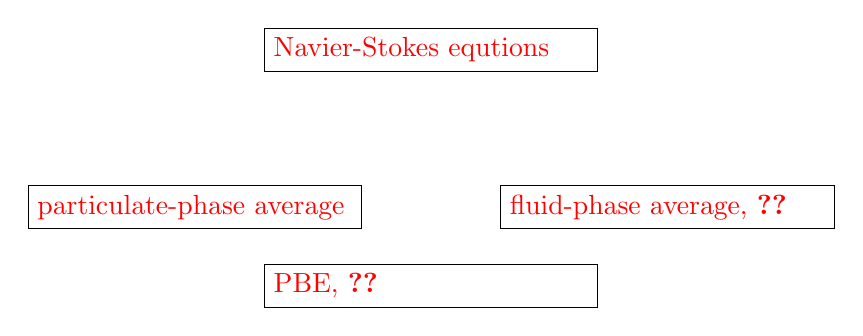
\begin{tikzpicture}
    \node[ell](pic1) at (0,0){Navier-Stokes equtions};
    \node[ell](pic2) at (3,-2){fluid-phase average,  \ref{eq:favgsp}};
    \node[ell](pic2) at (0,-3){PBE,  \ref{eq:PBM}};
    \node[ell](pic2) at (-3,-2){particulate-phase average};
\end{tikzpicture}






\section{The Closure problem}
\label{sec:closure}
The averaged equations derived previously all needs what we call closure terms to be solvable. 
In this section, we outline them from the lowest order to the higher ones.
Note that the importance of higher order terms become more and more important, as the suspension get nonuniform. 
Likewise, we start by revealing the closures of the fluid-phase average (\ref{eq:favgsp}) and particulate-phase average for rigid particles (\ref{eq:pavgsp}). 
Then, we discuss the implication of the deformable particle model on the closure terms. 
Lastly, the closure problem for the PBE (\ref{eq:PBM_QBMM}) will be discussed. 


\subsection{The averaged drag force $n\left<f\right>^p$}
This term shows up in both particulate-phase and fluid-phase average. 
It represents the drag force generated by the fluid phase on the dispersed phase.
Therefore, it appears with a minus sing in the fluid average and a positive sign in the particulate average.  
This term is of the most importance since it appear as it is, unlike the following terms which are under a divergence operator. 
Thus, accurate empirical formulas must be provided to predict its value for a set of dimensionless numbers ($Ga$, $Bo$, $\mu_r$, $\phi$), this is the aim of \ref{chap:DNS}. 
This force is composed of a hydrodynamical part $\bm{f}^h$ which is the drag force due to the stress of the fluid, a contact force $\bm{f}^{b}$.
Consequently, $\left<\bm{f}\right>^p=\left<\bm{f}^h\right>^p+\left<\bm{f}^b\right>^p$.
In dilute suspension the contact force vanish and closure for the hydrodynamical force can be found theoretically. 
Indeed, in 

\subsubsection{A single bubble or drop rising}
\paragraph*{Drag law for drops}
Theory from clift book
\paragraph*{Theory from \citet{tomiyama1998drag}}
The rise of a bubble (not a drop) can be correlated with the following dimensionless numbers :
\begin{align}
    Re = & \frac{\rho_L V_T d}{\mu_L}\\
    Eo = & \frac{g(\rho_L-\rho_D) d^2}{\sigma}\\
    M = & \frac{g\mu_L^4(\rho_L-\rho_G)}{\rho_L^2\sigma^3}\\
\end{align}
$Re$ is the non-dimensional velocity, $Eo$ compare the buoyancy to surface tension and $M$ is the property group of the two phases. 
Balance of drag and buoyancy forces :
\begin{equation}
    C_D 1/2 \rho_LV^2_T\frac{\pi d^2}{4}= (\rho_L-\rho_G)g\frac{\pi d^3}{6}
\end{equation}
\begin{equation}
    V^2_T = \frac{4(\rho_L-\rho_G)g d}{3C_D\rho_L},
\end{equation}
Then they define 3 regimes and different correlations. 
\paragraph*{Theory from \citet{loth2008drag}}
Most recent models for the Drag coefficient. 
\begin{itemize}
    \item \cite{tomiyama1998drag} propose some drag coefficient for bubbles. 
    \item \cite{sporleder2012population} summarize all the drag coefficient available.
    \item \citet{gemello2018modelling} summarize it too. They probably have the same. 
\end{itemize}
\subsection{The fluctuations terms}
In \ref{eq:favgsp}, \ref{eq:pavgsp} and \ref{eq:Iavg} we can note average of product of the fluctuations. 
Indeed, all the product of microscale variables $\left<\bm{uu}\right>$ can be rewritten as a product of average plus the average of fluctuations, namely $\left<\bm{uu}\right> = \left<\bm{u}\right>\left<\bm{u}\right> + \left<\bm{u'u'}\right>$. 
Each time this second order tensor appear under the divergence operator, therefore, this term is smaller than the averaged forces. 
Nevertheless, the velocity fluctuations have shown great importance in Euler-Euler simulation. 
\subsubsection{Turbulence and pseudo turbulence}
Rising bubbles often induce turbulence in the flow by different meaning. 
Since the velocity fluctuation plays a key role in the averaged equations it is of interest to study turbulence in details. 
\begin{itemize}
    \item The reference for the different scale of turbulence technics \citet{balachandar2009scaling}.
    They demonstrate that the point-particle approach is uniquely valid if the Kolmogorov timescale and particles timescale ratio is greater than one. $(\tau_p/\tau_k)>1$.  
    \item Distinguish the pseudo-Turbulence and pure-turbulence fluctuation. Show that it is the same phenomenon at two different timescale (look a flkin report and \citet{gemello2018modelling}\citep{mehrabadi2015pseudo}). 
    \item In bubbles suspension, at large Reynolds number the turbulence is caused by two sources \citep{risso2018agitation}. 
    Shear-induced turbulence (SIT) large-scale buoyancy-driven flows, and bubble-induced agitation (BIA). 
    They experimentally characterize those phenomenons.
    They obtain excellent  conclusion on velocity fluctuation. 
    \item The book Turbulence and Interaction. \citet{deville2009turbulence}. General concepts of turbulence. 
    \item \citet{du2022analysis} Although i'm not sure if it is about turbulence. 
\end{itemize}

\subsection{First and higher moments}
In the fluid-phase average, the last contribution to the bulk stress from the particles are the hydrodynamic moments.
In practice, even the first moment is rarely implemented in Euler-Euler models since it is not trivial to compute.
Therefore, we will only focus on the first moment and neglect the higher ones. 
As mentioned earlier the first moment tensor is the sum of a symmetric tensor called the stresslet, and of an antisymmetric one which is related to the torque.  
The mean stresslet has its importance in certain cases.
Indeed, when shear flow is dominant the divergence of this tensor become non-negligible.
For example, one can derive the expression of the bulk viscosity of a dilute suspension, by using the expression of the averaged stresslet tensor \citep{einstein1905neue}. 
In our case, with ascending droplets, it might be however negligible as there is no shear stress. However, the antisymmetric part of the first moment, or the averaged torque, might not be negligible.
Consequently, this term closure will be investigated in \ref{chap:DNS}.  







\subsection{The particle-fluid-particle stress}
\paragraph*{Particles-stress}

Full derivation of the particle stress which predict the particle migration in stoke flows:
\citet{nott2011suspension}

The nearest particle statistics (or particle-fluid-particles stress) which is the first order of the previous one:
\citet{zhang2021ensemble}
Derived a theoretical expression for the PFP stress based on the nearest particle probability. 

\citet{wang2021numerical}
The FPF stress calculated can periodic the drafting–kissing–tumbling mechanism. 
Thus, it can predict the macroscopic structure of the medium. 

 







\subsection{The source terms, $J(\mathcal{R},t)$.}
As said in the first part $J(\mathcal{\bm{R}},t)d\mathcal{R}$ is the rate of generation of entities. 
It encapsulates two phenomenons, the net rate of birth of entities $B(\mathcal{\bm{R}},t)d\mathcal{R}$ and the net rate of death of entities $D(\mathcal{\bm{R}},t)d\mathcal{R}$.
In droplet suspensions, we consider only one internal coordinate, $\lambda_0 = L$, the droplets size.
Then, $B$ and $D$ represent respectively the break-up and the coalescence of the droplets. 

Comparison of bubbles size distribution in zero gravity \citet{KAMP20011363}
Introduce the different closure terms that \citet{KAMP20011363} used and describe it in the letter paragraphs.

Coalescence kernels : \citet{morel2010comparison}
Introduces the product of the two terms.
\subsubsection{Probability of coalescence and Film drainage}
Make a scheme and introduce all the dimensionless number. 

\begin{itemize}
    \item \citet{chesters1991modelling} make a global overview of film drainage, time of coalescence and the overall coalescence Probability. The article mentions rigid and deformable particles. They investigate shear flow and turbulent flows too. Other specificity is referred as the interfacial-tension gradients.
    The probability reads as : $P = \exp(-\frac{t_d}{t_i})$
\end{itemize}
\begin{itemize}
    \item Diapo of JL. 
    \item The basis theory of film drainage \citet{jones1978film}
    \item On polydisperse suspension of drops, the common phenomenon is that one small drops merge with a bigger one due to different buoyancy (and thus velocity). 
    \citet{yiantsios1990buoyancy} analyzed with film drainage theory and boundary Integral method, the profile of deformation of the drop surface when getting close to a rigid interface.
    They solve  the problem by asymptotic matching analysis. 
    They conclude that a dimple is always formed and that the thinning rate $h\sim 1/t^\alpha$.
    \item In \cite{leal2004flow} they observe experimentally the film drainage of two drops. 
        They summarize all the literature available for film drainage.
        They could conclude that the film will tends to have a dimple since the pressure is maximum at the center.
        Likewise, they, also study polymer/surfactant effects 
    \item Derived equations of film drainage most recently \cite{leal2007advanced}
    \item thinning Viscoelastic film drainage equations are derived in \citet{bousfield1989thinning} 
    \item \citet{sambath2019inertial}  investigate the drop collision with numerical simulation.
    They consider Van-deer Val's forces in addition to inertial, capillarity and viscous forces.
    Thanks to a Lagrangian-eulerian method they can model length scale five order of magnitude below the radii length scale and resolve the film properly with Vandar wals forces. 
    They conclude that inertial delay the time of coalescence due to the bouncing between the two drops even tough the viscosity and density ratio is moderate. 
    The simulation carried out in this paper are asymmetric while most of the collisions aren't.
\end{itemize}
\paragraph*{for suspension}
\begin{itemize}
    \item \cite{zinchenko1994gravity} the y consider noo interia and poly-disperse suspension, with gravity induced suspension.
    It investigate the collision efficiency. 
\end{itemize}

\subsubsection{Collision frequency}

\begin{itemize}
    \item \citet{chesters1991modelling} provide us with a scaling law for collision frequency : $f\sim U D^2n^2$.
    \item \citet{davis1985sedimentation} (not sure it is the right article) provide collision frequency terms for buoyant suspension. 
    \item For turbulent flows  \citet{saffman1956collision} bring also a formulation.
    \item Nothing for the closure induce by bubbles.
    \item En regime de stokes closure are available, ask JL its in the diapo. 
    \item \citet{zhang1991rate} study the rate of collision for gravity induced collision.
    \item \citet{davis1984rate} study theoritically, the doublet of particles formed by Waader-vals interactions.
    For righid spherical particles, and compare to DNS. 
    The particles are sedimenting htough gravity. 
\end{itemize}
\subsubsection{Collision forces and duration}
It is of interest to identify the different hydrodynamic regime when particles get close to each other.
\begin{itemize}
    \item In the stokes regime, for rigid particles \citep{guazzelli2011} summarize the lubrication forces theories.  
    There are two main regimes, either the particles  are squeezing flow between them or shearing  it at constant velocity. 
    The former situation present a singularity when the particles touch each other, while the second configuration doesn't. 
    \item \cite{davis1989lubrication} present the theoretical framework for the resistance force of two squeezing spherical particles.
    They make use of both, boundary Integral Method  (BIM) \citep{pozrikidis1992boundary} and the lubrication theory.   
    They suppose three different situations : One where the particles are at moderate separation and/or high viscosity, and thus stay rigid. Then, they consider a deformable interface when the drops are relatively close and viscosity ratio low. Then they study the limits where the interface is fully mobile.  
    In each situation they conclude respectively that the force of resistance $F$ was :
    % $F\sim 1/d$ and  $F \sim \sqrt\{d}$. 
    They take as     hypothesis that the $(a/h) Ca\ll 1$
\end{itemize}


\paragraph*{Transition to DNS chap.} 
There is a lot of closure, while in the literature there is clearly a lake of closures. 